\documentclass[pdflatex,sn-mathphys-num]{sn-jnl}% Math and Physical Sciences Numbered Reference Style

\usepackage{graphicx}%
\usepackage{multirow}%
\usepackage{amsmath,amssymb,amsfonts}%
\usepackage{amsthm}%
\usepackage{mathrsfs}%
\usepackage[title]{appendix}%
\usepackage{xcolor}%
\usepackage{textcomp}%
\usepackage{manyfoot}%
\usepackage{booktabs}%
\usepackage{algorithm}%
\usepackage{algorithmicx}%
\usepackage{algpseudocode}%
\usepackage{listings}%

\theoremstyle{thmstyleone}%
\newtheorem{theorem}{Theorem}%
\newtheorem{proposition}[theorem]{Proposition}% 

\theoremstyle{thmstyletwo}%
\newtheorem{example}{Example}%
\newtheorem{remark}{Remark}%

\theoremstyle{thmstylethree}%
\newtheorem{definition}{Definition}%

\raggedbottom

\begin{document}

\title[CNNs for Hand Gesture Recognition]{An Empirical Study of Convolutional Neural Networks for Hand Gesture Recognition}

\author{\fnm{Alex} \sur{Tulip}}

\abstract{This paper presents my project on building a Convolutional Neural Network (CNN) to classify Rock-Paper-Scissors hand gestures. Following standard machine learning steps, I looked at how making the model more complex and using regularization techniques affects its performance. I designed three models, starting with a simple one and then adding more layers, dropout, and data augmentation. My results show that my first, simple model overfit the data badly. Adding regularization, especially data augmentation, was very helpful in fixing this. My final model got 97.7\% accuracy on the test data it had never seen before. To push it further, I tested it on my own pictures taken with my phone. This test showed that the model struggles with new types of images, which is an important thing to think about for real-world use. This project was a good way to see important machine learning ideas in action, like the trade-off between bias and variance and why it's important to have a clear plan.}

\maketitle

\section{Introduction}\label{sec1}

Image classification is a key part of modern machine learning, and Convolutional Neural Networks (CNNs) are one of the best methods for these kinds of tasks. In this project, I tried to classify images from the Rock-Paper-Scissors dataset, which contains pictures of the three hand gestures. My main goal wasn't just to get the highest accuracy possible, but to really understand the process of building a good CNN model using the ideas I learned in class.

As we learned in our course notes~\cite{cesa2024smml}, building a good model involves finding the right balance between bias and variance. If a model is too simple, it might underfit the data (high bias) and not learn the important patterns. If it's too complex, it might overfit (high variance) by basically memorizing the training data, noise and all, which means it won't do well on new images. This project looks at this trade-off directly by building and testing three different CNNs, each one a bit more complex than the last.

I wanted to answer these questions:
\begin{enumerate}
    \item How does making a model more complex affect its performance on an image classification task?
    \item How well do common techniques like Dropout and data augmentation work to stop overfitting and help the model generalize?
    \item How well does a model that is very accurate on its test set perform when it's given completely new images from a different source?
\end{enumerate}

I'll go through how each model performed by looking at its training and validation graphs. I'll use regularization to try and control the model's complexity and make it better at generalizing. The best model is then tested on a final, held-out test set to get a fair measurement of how well it would perform on new data.

\section{Methods}\label{sec11}

I tried to set up my project in a clear and organized way so that someone else could repeat it. I used standard practices for machine learning projects. The whole project was done in Python using TensorFlow and Keras, and I ran my code on a T4 GPU in Google Colab.

\subsection{Dataset and Preprocessing}
I used the Rock-Paper-Scissors dataset from Kaggle~\cite{kaggle_rps}. It has 2,188 color images of hand gestures, with a good balance between the three classes: 'rock', 'paper', and 'scissors'. The pictures are 300x200 pixels and have different backgrounds and lighting.

First, I split the data into three separate parts: a training set (60\% of the data), a validation set (20\%), and a test set (20\%). It's important to split the data this way to avoid the model accidentally learning from the test data, which would make the final evaluation unfair. The validation set is for tuning the model, and the test set is only used once at the very end to see how the final model does. The number of images in each set is in Table~\ref{tab:split}.

\begin{table}[htbp]
\caption{Dataset split counts}\label{tab:split}%
\begin{tabular}{@{}lcccc@{}}
\toprule
Set & Rock & Paper & Scissors & Total \\
\midrule
Training & 435 & 427 & 450 & 1312 \\
Validation & 145 & 142 & 150 & 437 \\
Test & 146 & 141 & 152 & 439 \\
\botrule
\end{tabular}
\end{table}

Before feeding the images to the model, I resized them all to 150x150 pixels. I also normalized the pixel values from the [0, 255] range to a [0, 1] range by dividing by 255. This is a standard step that helps the neural network train more easily.

\subsection{Model Architectures}
I designed three CNN models, each one a bit more complex than the last, to see how the changes would affect performance.

\subsubsection{Model 1: Baseline CNN}
My first model was a very simple CNN. I used it to get a baseline result and to see how a simple model would behave. It has one convolutional layer and one dense layer.
\begin{itemize}
    \item \texttt{Conv2D} (16 filters, 3x3 kernel, ReLU activation)
    \item \texttt{MaxPooling2D} (2x2 pool size)
    \item \texttt{Flatten}
    \item \texttt{Dense} (64 units, ReLU activation)
    \item \texttt{Dense} (3 units, Softmax activation for output)
\end{itemize}
I chose a small number of filters (16) to keep the model's capacity low, which I thought would make it easier to see the learning process clearly.

\subsubsection{Model 2: Intermediate CNN with Dropout}
To try and fix some of the problems I saw with the first model, my second model was deeper and used regularization. I increased the number of filters in the convolutional layers (first 32, then 64) so the network could learn more complex features.
\begin{itemize}
    \item \texttt{Conv2D} (32 filters, 3x3 kernel, ReLU activation)
    \item \texttt{MaxPooling2D} (2x2 pool size)
    \item \texttt{Conv2D} (64 filters, 3x3 kernel, ReLU activation)
    \item \texttt{MaxPooling2D} (2x2 pool size)
    \item \texttt{Flatten}
    \item \texttt{Dropout} (rate of 0.5)
    \item \texttt{Dense} (128 units, ReLU activation)
    \item \texttt{Dense} (3 units, Softmax activation)
\end{itemize}
The most important addition here is the \texttt{Dropout} layer. This helps prevent overfitting. It works by randomly "turning off" half of the connections in the layer during training. This forces the model to learn in a more robust way and not rely too much on any single neuron.

\subsubsection{Model 3: CNN with Data Augmentation}
My third model has the same structure as Model 2, but I trained it using data augmentation to help it generalize even better. I set up the training data generator to apply random changes to the images as they were being fed to the model:
\begin{itemize}
    \item Rotation (up to 20 degrees)
    \item Width and height shifts (up to 20\%)
    \item Shearing and zooming (up to 20\%)
    \item Horizontal flipping
\end{itemize}
This technique basically creates more training data for free. By showing the model slightly changed versions of the same images, it learns to recognize the hand gestures no matter their position or orientation.

\subsection{Training and Evaluation}
I trained all three models using the Adam optimizer, which is a popular and effective way to train these models. I used the \texttt{categorical\_crossentropy} loss function because it's the standard for this type of classification problem, and I tracked accuracy during training. For my final model, I did a quick search for the best learning rate ($10^{-3}$ or $10^{-4}$), picking the one that did best on the validation set.

\section{Results}\label{sec2}

I trained the three models and recorded their training and validation accuracy over time.

\subsection{Model 1: Baseline Performance and Overfitting}
The baseline model trained fast. It got to 99.3\% accuracy on the training data, but its validation accuracy was only 95.2\%. The learning curves in Figure~\ref{fig:model1} showed a big gap opening up between the training and validation accuracy. This is a classic sign of **overfitting**: the model has learned the training data perfectly, but it can't generalize to new images. This means the model has low bias (it can fit the training data) but high variance (it doesn't generalize well).

\begin{figure}[htbp]
\centering
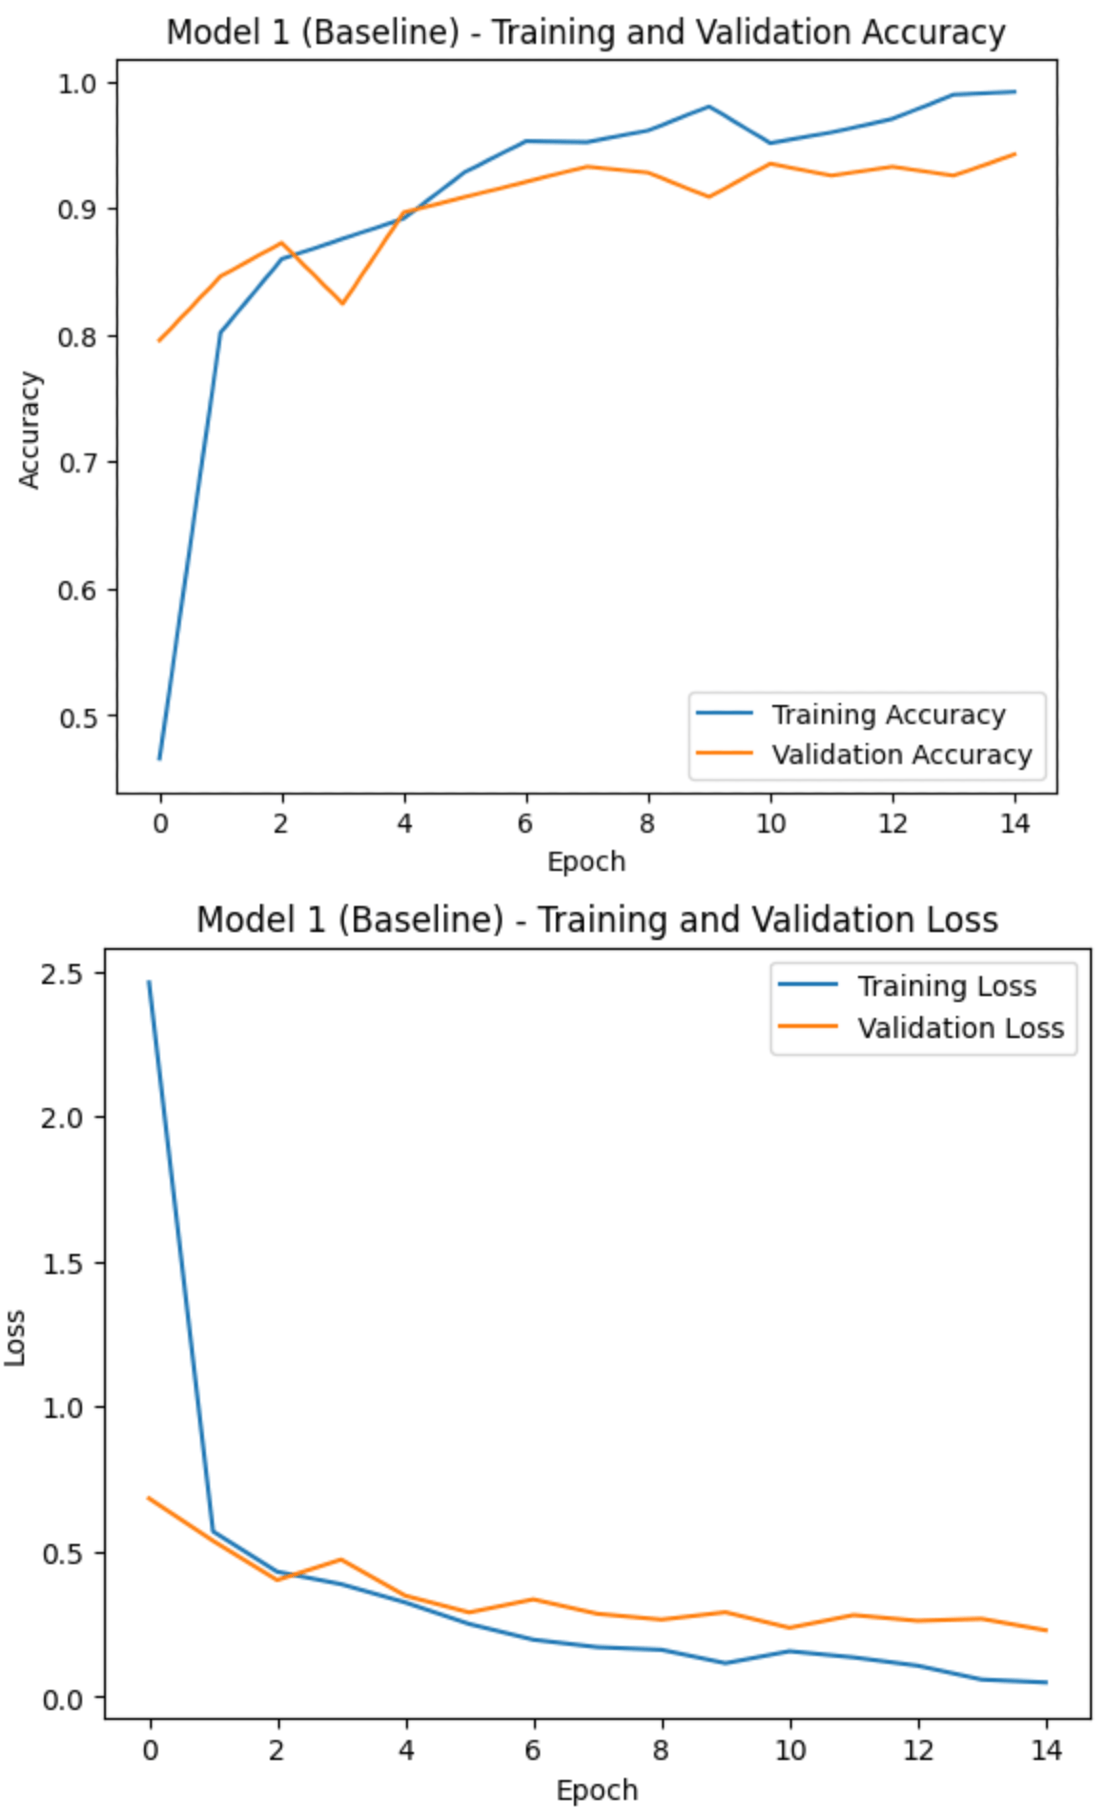
\includegraphics[width=0.9\textwidth]{model1_curves.png}
\caption{Training and validation accuracy/loss for Model 1. The growing gap between the training and validation curves indicates significant overfitting.}\label{fig:model1}
\end{figure}

\subsection{Model 2: The Effect of Dropout}
The second model, which had an extra convolutional layer and a dropout layer, did better. It reached a validation accuracy of 96.2\%. As you can see in Figure~\ref{fig:model2}, the gap between the training and validation curves is much smaller than in the first model. This showed that dropout helped to regularize the model and made it generalize better.

\begin{figure}[htbp]
\centering
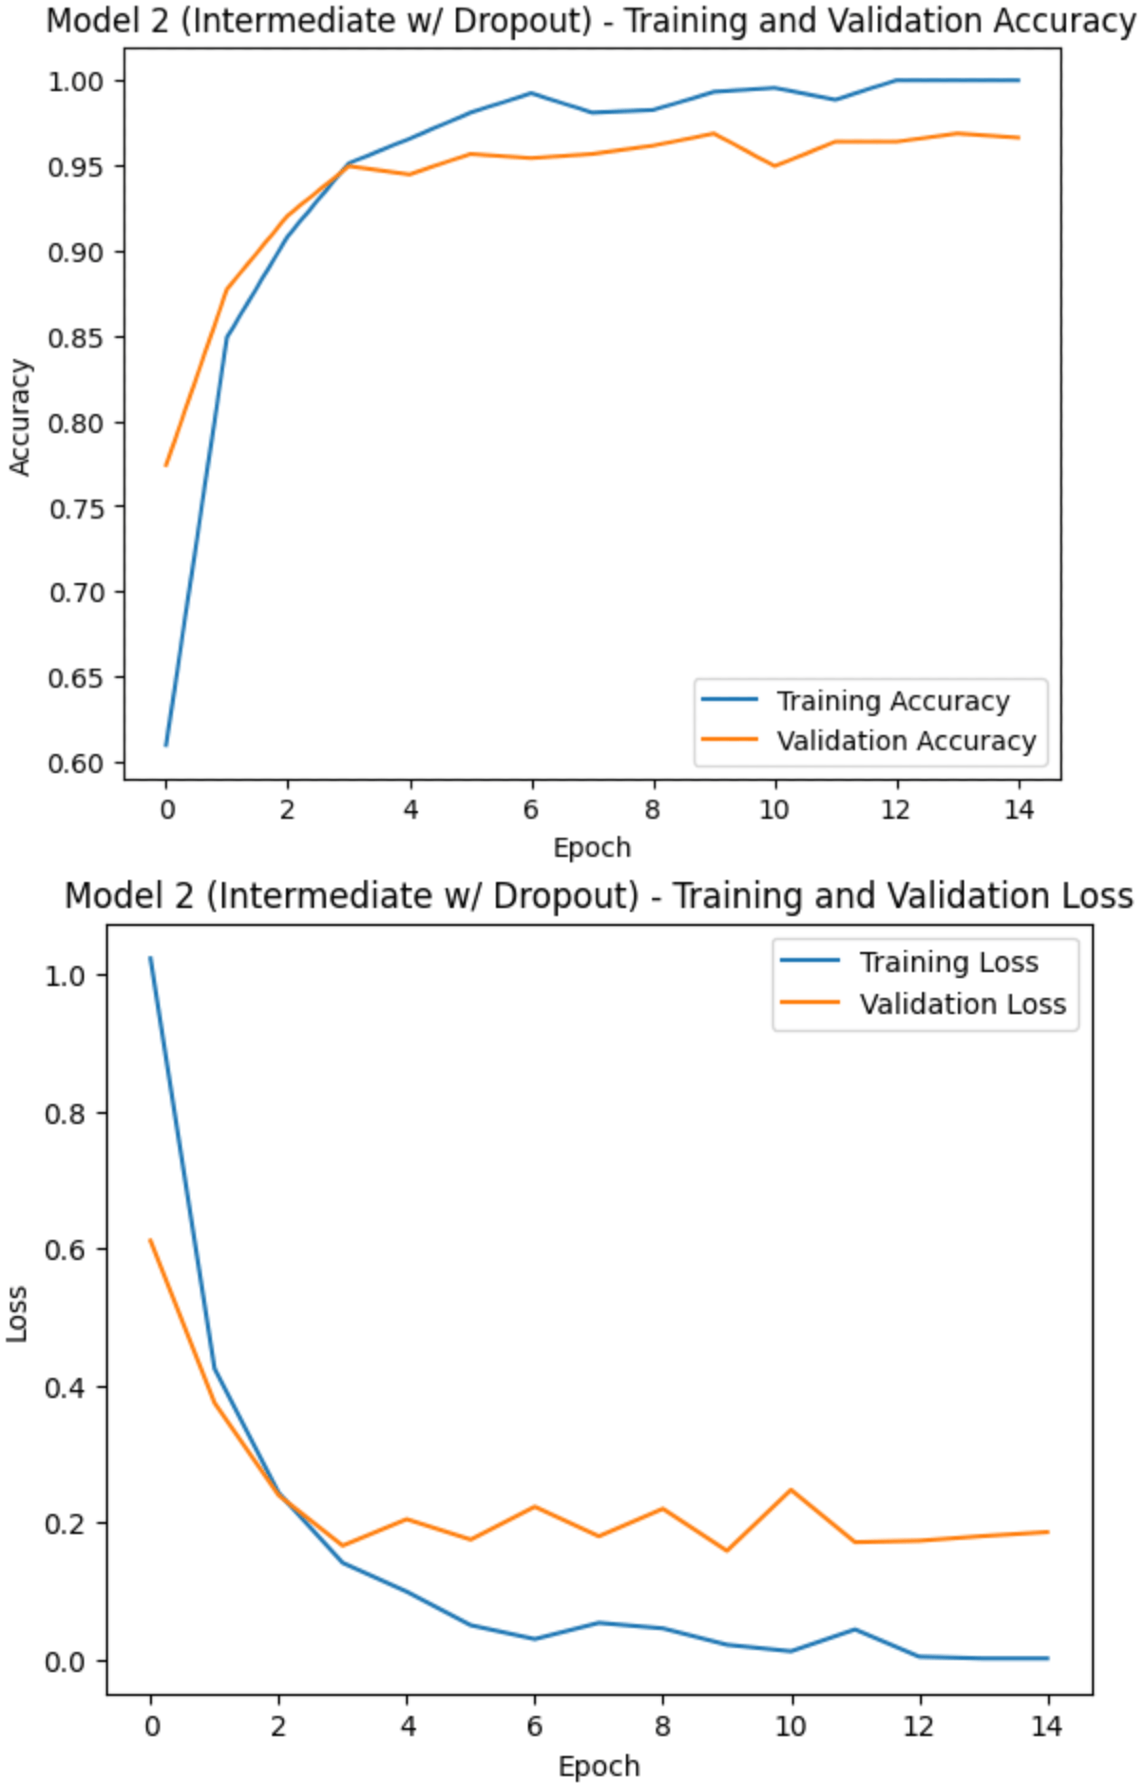
\includegraphics[width=0.9\textwidth]{model2_curves.png}
\caption{Training and validation accuracy/loss for Model 2. The gap between the curves is reduced, showing that dropout has mitigated some overfitting.}\label{fig:model2}
\end{figure}

\subsection{Model 3: The Power of Data Augmentation}
The third model, which I trained with data augmentation, gave me the best results. It reached a validation accuracy of 98.6\%. In Figure~\ref{fig:model3}, the training and validation curves follow each other very closely. This shows that overfitting is no longer a big problem and the model generalizes very well. The training accuracy is now much closer to the validation accuracy, which is what you want to see in a well-balanced model.

\begin{figure}[htbp]
\centering
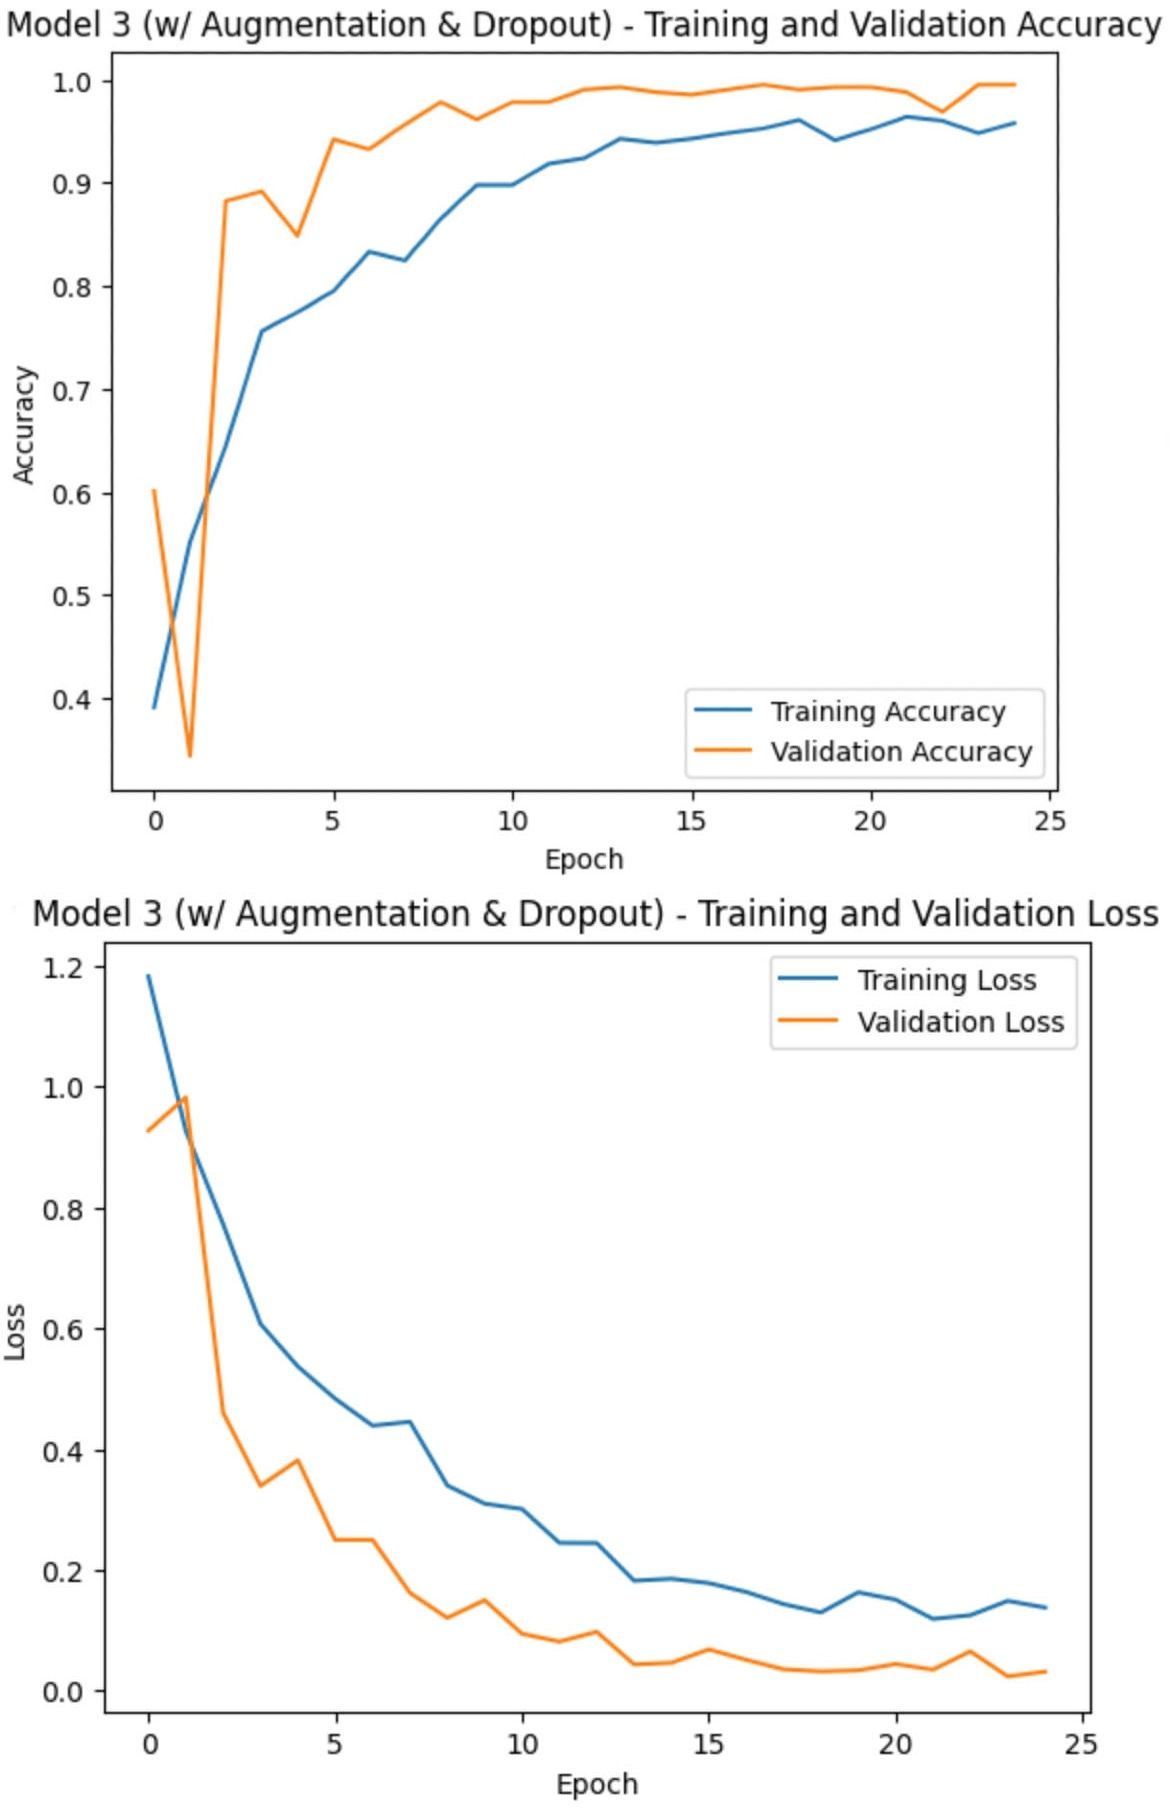
\includegraphics[width=0.9\textwidth]{model3_curves.png}
\caption{Training and validation accuracy/loss for Model 3. The curves are closely aligned, indicating a well-regularized model with excellent generalization.}\label{fig:model3}
\end{figure}

\subsection{Final Model Evaluation}
After choosing the best model (Model 3's architecture with data augmentation), I trained it one last time and tested it on the held-out test set. This gives me a final, fair score for the model. The model achieved a **test accuracy of 97.72\%**. The detailed report is in Table~\ref{tab:report}, and the confusion matrix is in Figure~\ref{fig:cm}.

\begin{table}[htbp]
\caption{Classification Report for the Final Model on the Test Set}\label{tab:report}%
\begin{tabular}{@{}lcccc@{}}
\toprule
Class & Precision & Recall & F1-Score & Support \\
\midrule
rock     & 0.99 & 0.94 & 0.96 & 141 \\
paper    & 0.95 & 1.00 & 0.97 & 150 \\
scissors & 0.99 & 0.99 & 0.99 & 148 \\
\midrule
Accuracy &      &      & 0.98 & 439 \\
Macro Avg & 0.98 & 0.98 & 0.98 & 439 \\
Weighted Avg & 0.98 & 0.98 & 0.98 & 439 \\
\botrule
\end{tabular}
\end{table}

\begin{figure}[htbp]
\centering
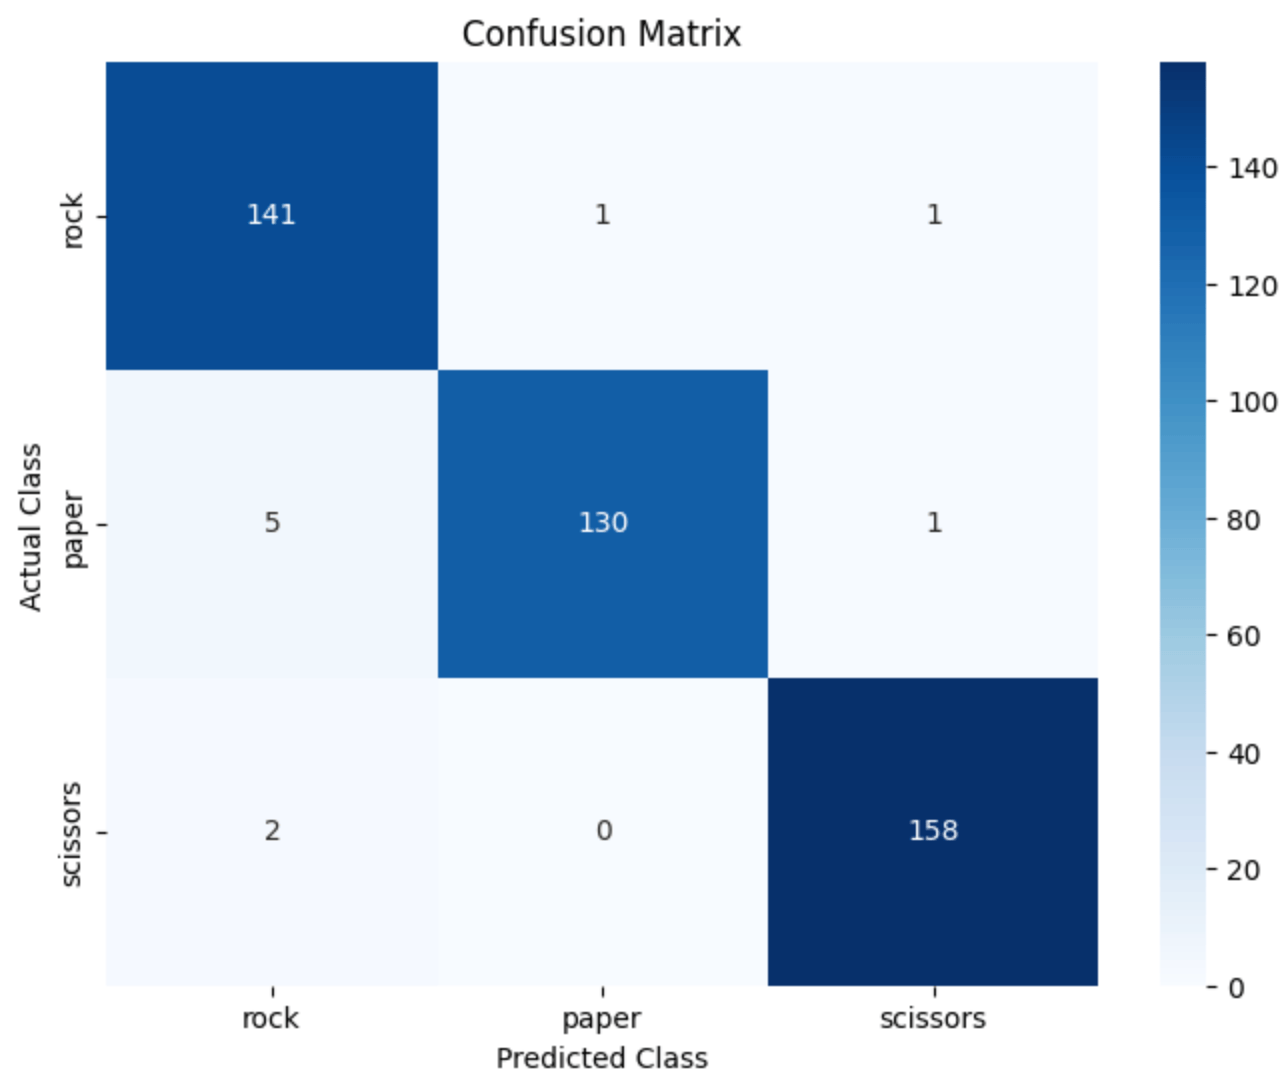
\includegraphics[width=0.6\textwidth]{confusion_matrix.png}
\caption{Confusion matrix for the final model on the test set. The model shows high accuracy across all classes, with the most frequent error being the misclassification of 'rock' as 'paper'.}\label{fig:cm}
\end{figure}

\subsection{Generalization Test on Custom Images}
To test the model even more, I made a small set of 6 of my own images (2 of each gesture) using my phone camera. I purposely took these pictures in different conditions, with real backgrounds and normal lighting, to see how the model would handle images that were different from its training data.

The model did much worse on these new pictures. It got the 2 'paper' images right, but it thought all of my 'rock' and 'scissors' pictures were also 'paper'. This means it only got an accuracy of **33.3\%** (2 out of 6 correct). The model was also very confident about its wrong answers, which shows a common problem with neural networks when they see data that is different from what they were trained on.

\section{Discussion}\label{sec12}

This project was a good exercise in building a CNN classifier in a structured way. Going from the simple model that overfit to the final, better model really showed how important ideas from class, like regularization, are in practice.

My first baseline model was a clear case of high variance. I fixed this by adding regularization. Model 2 showed that dropout can help, but the biggest improvement by far came from Model 3 with data augmentation. By creating lots of slightly different training images, I made the model learn the general features of the hand gestures, which made it much better at generalizing.

Getting 97.7\% on the test set was a great result, but the most interesting part was testing it on my own pictures. The accuracy dropped to 33.3\% on my 6 custom images. This is a classic example of what's called **domain shift**: a model that works great on data from one source fails when it's given data from another. The model probably learned features that were specific to the Kaggle dataset, like the plain backgrounds and studio-style lighting, instead of just the abstract shape of the hand. This is a good reminder that even a model with a high test score might not work well in the real world unless it's trained on a much wider variety of data. For a real application, I would need to gather a lot more training images from different places, or maybe use more advanced techniques to help it adapt.

\section{Conclusion}\label{sec13}

In this project, I built a Convolutional Neural Network that can classify Rock-Paper-Scissors gestures with high accuracy. By starting with a simple model and then adding complexity and techniques like dropout and data augmentation, I was able to fix the initial problem of overfitting and make the model generalize much better. My final model got an accuracy of 97.7\% on the test set. However, a final test on my own photos showed that the model struggles when the images are different from its training data, which is an important weakness to consider for any real-world use. Overall, this project was a great hands-on way to use the main ideas of machine learning to build and test a deep learning model.

\backmatter

\begin{appendices}

\section{Model Summaries}\label{secA1}

This appendix contains the detailed architecture summaries for the three models, as generated by Keras.

\subsection{Model 1 Summary}
\begin{verbatim}
Model: "sequential"
_________________________________________________________________
 Layer (type)                Output Shape              Param #   
=================================================================
 conv2d (Conv2D)             (None, 148, 148, 16)      448       
                                                                 
 max_pooling2d (MaxPooling2D) (None, 74, 74, 16)       0         
                                                                 
 flatten (Flatten)           (None, 87616)             0         
                                                                 
 dense (Dense)               (None, 64)                5607488   
                                                                 
 dense_1 (Dense)             (None, 3)                 195       
                                                                 
=================================================================
Total params: 5,608,131
Trainable params: 5,608,131
Non-trainable params: 0
_________________________________________________________________
\end{verbatim}

\subsection{Model 2 Summary}
\begin{verbatim}
Model: "sequential_1"
_________________________________________________________________
 Layer (type)                Output Shape              Param #   
=================================================================
 conv2d_2 (Conv2D)           (None, 148, 148, 32)      896       
                                                                 
 max_pooling2d_2 (MaxPooling  (None, 74, 74, 32)        0         
 2D)                                                             
                                                                 
 conv2d_3 (Conv2D)           (None, 72, 72, 64)        18496     
                                                                 
 max_pooling2d_3 (MaxPooling  (None, 36, 36, 64)        0         
 2D)                                                             
                                                                 
 flatten_1 (Flatten)         (None, 82944)             0         
                                                                 
 dropout (Dropout)           (None, 82944)             0         
                                                                 
 dense_2 (Dense)             (None, 128)               10616960  
                                                                 
 dense_3 (Dense)             (None, 3)                 387       
                                                                 
=================================================================
Total params: 10,636,739
Trainable params: 10,636,739
Non-trainable params: 0
_________________________________________________________________
\end{verbatim}

\subsection{Model 3 Summary}
The architecture for Model 3 is identical to Model 2. The difference lies in the training data, which was augmented as described in the Methods section.

\end{appendices}


\begin{thebibliography}{9}

\bibitem{cesa2024smml}
Cesa-Bianchi, N. (2024). *Course Notebook: Statistical Methods for Machine Learning*. University of Milan.

\bibitem{kaggle_rps}
Dr. G. Freeman. (2019). Rock Paper Scissors Dataset. Kaggle. \url{https://www.kaggle.com/datasets/drgfreeman/rockpaperscissors}

\end{thebibliography}

\end{document}